\documentclass{article}
\usepackage{subcaption}
\usepackage[utf8]{inputenc} % allow utf-8 input
\usepackage[T1]{fontenc}    % use 8-bit T1 fonts
\usepackage{hyperref}       % hyperlinks
\usepackage{url}            % simple URL typesetting
\usepackage{booktabs}       % professional-quality tables
\usepackage{amsfonts}       % blackboard math symbols
\usepackage{nicefrac}       % compact symbols for 1/2, etc.
\usepackage{microtype}      % microtypography
\usepackage{lipsum}

% monospace like in stackoverflow
\usepackage{xcolor}
\definecolor{light-gray}{gray}{0.95}
\newcommand{\code}[1]{\colorbox{light-gray}{\texttt{#1}}}

% Alternative
\NewDocumentCommand\huggingface{}{
    
\includegraphics[scale=0.04]{huggingface.png}
}

\setlength{\parindent}{0cm}

\usepackage{graphicx}
\usepackage{caption}
\usepackage{subcaption}
\usepackage{amsmath}
% Used for displaying a sample figure. If possible, figure files should
% be included in EPS format.
%
% If you use the hyperref package, please uncomment the following line
% to display URLs in blue roman font according to Springer's eBook style:
% \renewcommand\UrlFont{\color{blue}\rmfamily}

\begin{document}
%
\title{Question Answering and Information Retrieval on the SQuAD Dataset}

\author{
Francesco Rambaldi \and Daniele Verì \and Luca Serfilippi \and Marco Buiani \\
\texttt{name.surname@studio.unibo.it}
}

\date{}

\maketitle

\begin{abstract}
Question Answering (QA) is a challenging neural comprehension task which requires a system to reason simultaneously on two segments of text, namely a question and the paragraph in which to find the answer. In this project work we tackle QA and test two different neural architectures on it. We implement a model based on Recurrent Neural Networks and fine tune variations of a Language Model based on Transformers. We experiment with modifications on the two main network structures and compare the results on the SQuAD dataset.
We then implement an Information Retrieval (IR) model with the aim of combining it with our QA module. Our work on IR focuses on two main methods, one based on tf-idf, and the other based on a neural architecture (Transformer). We developed the IR module in parallel with the QA component, while we decide to merge them after accurate evaluation of both parts. 
The final part of our work consists in the deploy of a complete IR-QA system on the Google Cloud Platform.
\end{abstract}\hspace{10pt}

%\keywords{Question Answering  \and Information retrieval \and Transformers \and BERT \and RNN}

\section{Question Answering}

The question answering task proposed in the SQuAD dataset is defined as the problem of providing a single answer to a question, obtained by selecting a span of text from the related paragraph.
This is a specific kind of factoid question answering where the reading comprehension system is given a query-passage pair in input. 

\subsection{Dataset split}\label{dataset_split}
The SQuAD dataset is composed by two json files: the \code{trainset} and \code{devset}. We use the \code{devset} as test data while we split the \code{trainset} so that 10\% is used as validation data.

\subsection{Error Removal from the SQuAD dataset}
The first necessary step for working on the QA task with a neural architecture is preprocessing (and tokenization) of each question and answer. In order to perform this in the best possible way, we analyzed in depth the structure of the dataset. During this analysis we found out that the SQuAD 1.1 dataset contains various errors (this is probably due to the way in which the question-answer pairs were gathered in its creation, namely by crowdsourcing).
In the following we list the main errors typologies we were able to spot in the SQuAD 1.1 dataset:

\begin{enumerate}
    \item The question/answer is incorrect (doesn't make any sense). Example:
    
    ID: 57262473271a42140099d4e9
    
    Question: "dd"
    
    Answer: "yptian Se"
    
    \item The provided answer is correct but truncated, thus it is not possible to find it in the tokenized text. Example:
    
    ID: 56bf7e603aeaaa14008c9681
    
    Question:  "What event caused Beyonce's depression?"

    Answer: "split with Luckett and Rober"

    Passage: "[...] Beyoncé experienced depression following the split with Luckett and Roberson after being publicly blamed by the media, critics, and blogs for its cause. [...]"
    
    The answer is almost correct but "Roberson" is truncated to "Rober" at the end.
    
    \item The provided answer is correct, but the related passage indices of start/end point to a wrong occurrence of the answer in the text. Example:
    
    ID: 56ccde7862d2951400fa64d9
    
    Question: "Who had a large amount of contacts with china during Yuan?"

    Answer: "Tibet"

    Passage: "[...] the reliability of the heavily censored History of Ming as a credible source on Sino-Tibet[1]an relations is questionable, in the light of modern scholarship. [...] Morris Rossabi also writes that "Tibet [2], which had extensive contacts with China during the Yuan, scarcely had diplomatic relations with the Ming."
    
    
    In this example, the answer indices point to [1], while they should point to [2].
    
    \item The provided answer is correct but written using letters instead of numbers (or vice-versa). As a consequence, the start/end indices point to a wrong occurrence in the text. Example:
    
    ID: 56cbdea66d243a140015edae
    
    Question: "At what age did Frédéric start giving public concerts?"

    Answer: "7"
    
    Passage: "[...] By the age of seven [1] Fryderyk had begun giving public concerts, and in 1817[2] he composed two polonaises, in G minor and B-flat major. [...]"
    
    In this example, the answer indices point to [2], while they should point to [1], which is the true answer to the question.
\end{enumerate}

We individuated over 240 such errors in the dataset, so we proceeded by eliminating the corresponding question/answer pairs. Then we performed preprocessing and tokenization.

\subsection{RNN System Description}
\subsubsection{Preprocessing}\label{preprocessing_for_RNN}
In order to exploit the pretrained GLoVE word embeddings~\cite{pennington2014glove}, the cleaned dataset is preprocessed with the aim of reducing the OOV word count.
The main problem to solve is the fact that we can have symbols or numbers not spaced from words, this will form s unique word and putting it OOV. Since symbols and numbers are contained into the GLoVE embedding we use regex formulas to split these words:
\begin{itemize}
    \item symbols regex:
    \code{re.sub(r"([$symbols$])", r" \symbol{92}1 ", text)}
    
    \item numbers regex:
    \code{re.sub(r"(\symbol{92}d+)([a-z]+)", r"\symbol{92}1 \symbol{92}2", text)}
    
    \item elimination of consecutive spaces:
    \code{re.sub(r"\symbol{92}s\{2,\}", r" ", text)}
\end{itemize}
The text is then tokenized, splitting each string by space. 
We create the train vocabulary using both train and validation set and we add the \code{[PAD]} token at index 0. Since during validation it's already evident that the Transformer models outperforms the RNNs, we don't build a test vocabulary and don't handle the unknown symbol via the \code{[UNK]} token.
Finally the GLoVE embedding matrix is merged with the train/val OOV words that are embedded with uniformly random vectors.
This matrix is used to initialize the weights of the embedding layer of our model.

\subsubsection{Model}
Recurrent Neural Networks have shown great potential for the processing of sequential data, for this reason we decide to use RNNs as feature extractors in our QA system,in particular LSTMs ~\cite{lstm}. The interaction between question and passage is then modeled by the query-value attention mechanism.

Figure~\ref{fig_1} describes the architecture of our model, to be read top to bottom.

\begin{figure}[h]
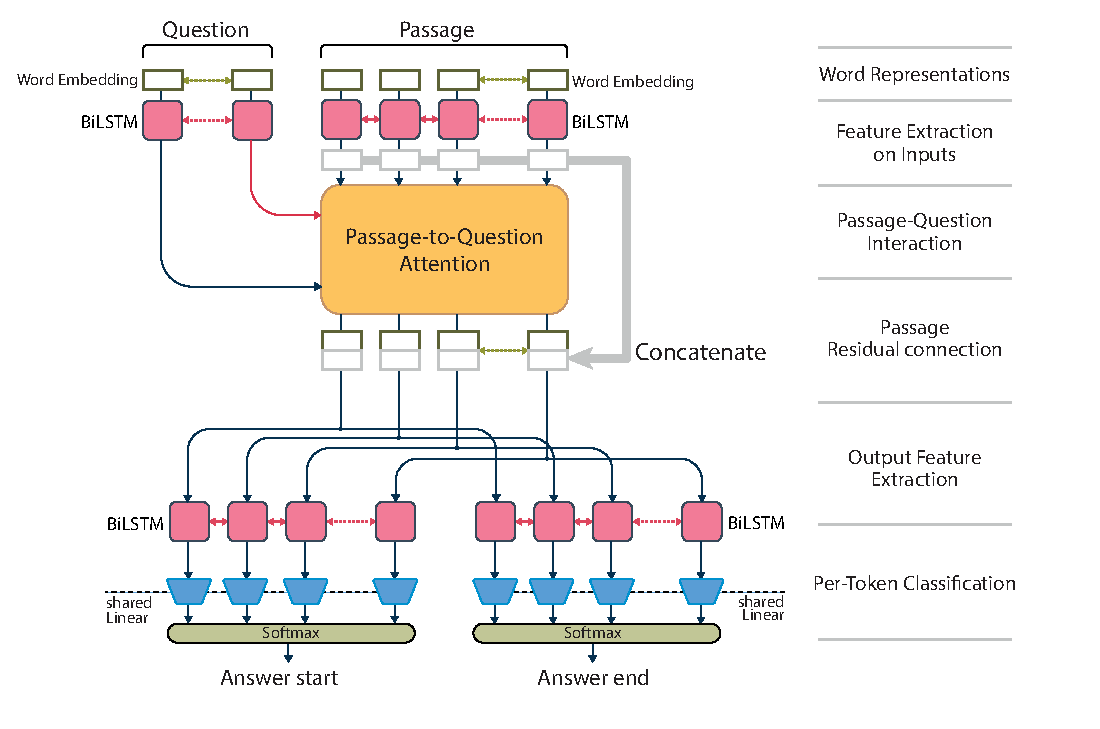
\includegraphics[width=\textwidth]{RNN_graph.eps}
\caption{RNN Attention model for QA.} \label{fig_1}
\end{figure}

A detailed description of our model follows: 

\begin{enumerate}
  \item Questions and passages are tokenized and encoded with GLoVE word vectors.
  \item Input passage and question are processed by two separate bidirectional LSTM layers.
  \item Hidden states of both inputs at each timestep are processed by dot product attention between question and answer. This produces an output with an embedding vector for each token in the original passage sequence.
  \item Attention output is concatenated to the previous LSTM states for passage.
  This "information highway" lets following layers see the passage tokens unaltered from attention.
  \item Two identical and independent classification heads process the concatenated stream to provide separate answer token start and end positions. Each implements a BiLSTM layer followed by a dense layer with softmax activation.
\end{enumerate}

It is important to to note how attention is performed between a question and passage: we use the passage as the query, where the question is the value.
This provides an output of the same shape as the passage input, thus retaining per-token information.
This mimics the expected behavior of reading the question in order to find an answer inside the passage.

\subsubsection{Experimental Setup and Results}

We evaluate our model based on the exact match metric, common to all our Question Answering models.
We also keep track of implementation specific metrics to help us in model design.\\

We halt the training with early stopping based on validation loss and a patience of 2 epochs, keeping the best model. No other form of regularization is employed.\\

We first train and evaluate the model described above:
the separate start-end heads are identical: the model is trained with categorical cross-entropy loss, computed on all possible token positions in the sequence, then summed equally for answer start-end tokens.
We call this the RNN classification configuration.\\

Results are presented for the best model on validation set.\\

The model achieves 30.52\% exact match.
We keep track of start and end accuracy metrics as well:
accuracy on answer start token: 40.18\%
accuracy on answer end token:   43.43\%

\subsubsection{Analysis of results}
\hfill \break
By constructing a start-end absolute positions plot for all predictions we see a clear clustering of answer points near the diagonal: this means that short answers are commonly well predicted. %\cite{fig2}

\begin{figure}[!ht]
\begin{subfigure}{0.5\textwidth}
\centering
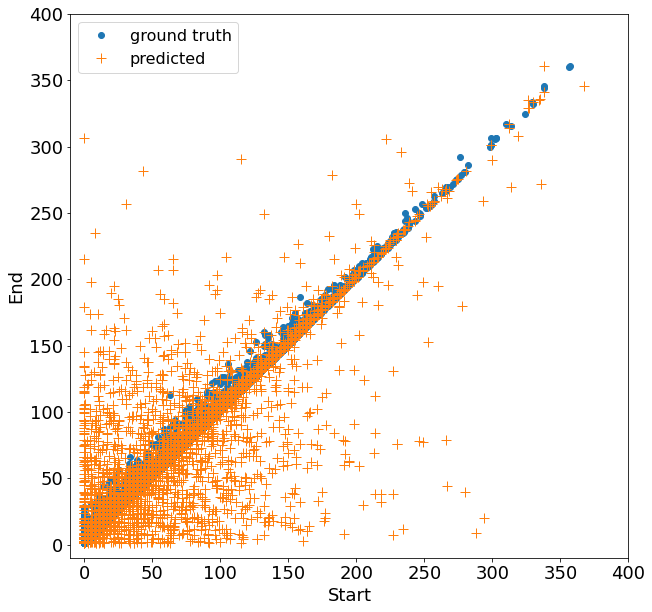
\includegraphics[width=1\textwidth]{RNN_classification_precedence.png}
\caption{Classification}
\label{fig2:sub1}
\end{subfigure}%
\begin{subfigure}{0.5\textwidth}
\centering
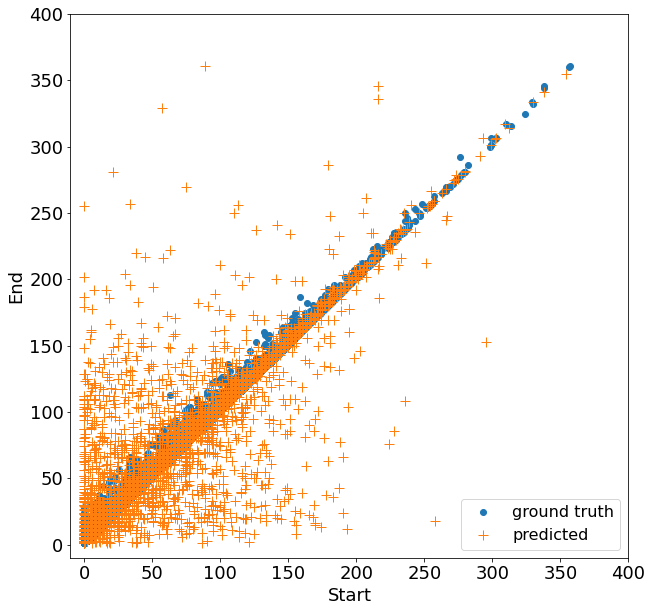
\includegraphics[width=1\textwidth]{RNN_constraint_precedence.png}
\caption{Custom Loss}
\label{fig2:sub2}
\end{subfigure}
\begin{subfigure}{\linewidth}
\centering
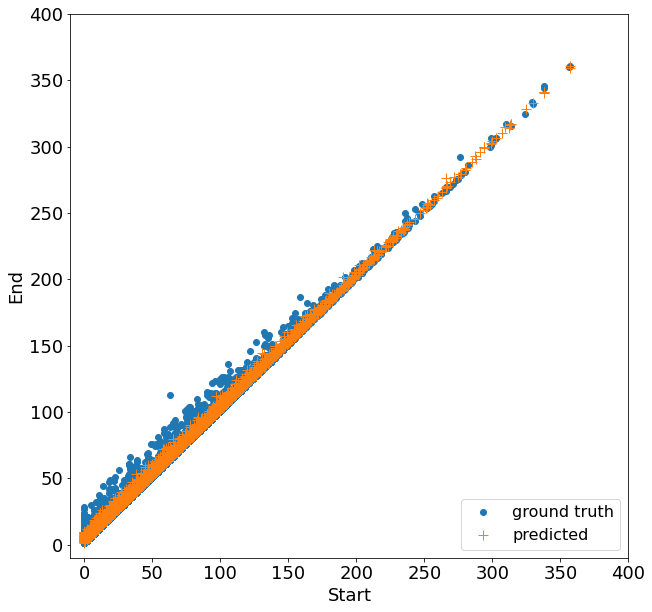
\includegraphics[width=.5\textwidth]{RNN_regression_precedence.png}
\caption{Regression}
\label{fig2:sub3}
\end{subfigure}
\caption{Precedence plots for RNN approaches}
\label{fig2}
\end{figure}

However, an unwanted behavior clearly emerges: in a consistent part of the predictions the start token follows the end one.
This happens for 11.33\% of prediction pairs.

This unsatisfactory result can be explained by the network construction: it predicts start-end positions independently and has no obligation to follow the common sense intuition of precedence.

Therefore, we inject this prior knowledge on the problem in the network in two different ways:  Answer length regression and Custom Loss.
\begin{itemize}
    \item In the first experiment we modify the end-token classification by adding a dense layer and ReLU activation so to perform answer length regression. Start cross-entropy classification loss and Mean Absolute Error end loss are summed equally.
    
    \item In a second modification we add a precedence term to the cross-entropy loss: \[L_{precedence} = \beta * max(start_p - end_p, 0)\]
    Precedence is positive when end position precedes start, while it goes to zero for correctly ordered pairs.
    This softly guides the network in achieving good precedence.
    
\end{itemize}

We report metric results for the three separate runs.


\begin{table}[h]
\centering
\caption{Comparison of results for RNN approaches}\label{tab1}

\begin{tabular}{| c | c | c |}
\hline
Model &  Exact Match & Precedence Violation\\
\hline
RNN classification &  30.52\% & 11.33\%\\

\hline
RNN regression &  18.85\% & 0.0\%\\

\hline
RNN custom loss &  32.54\% & 9.93\%\\

\hline
\end{tabular}
\end{table}

The precedence plot guided us into better understanding of the behavior of our model.
We try the regression approach as to remove the issue completely.
Unfortunately, this results in a worse performing model in terms of exact match.
Our hypothesis lies in the more difficult task devolved to the answer length head, who is not as easy as token classification.

Our custom loss approach manages to improve the exact match metric while also improving the precedence.
We think this is due to the more gentle injection of the prior into the loss, without twists of the cross-entropy loss.

\pagebreak

\subsection{System Description: Transformers}
The LSTM approach manages to achieve significant results on the SQuAD task with a balanced amount of resources.
However, we decide to improve the model performance following state-of-the-art methods based on transformers~\cite{vaswani2017attention}.

Recent works have shown that attention is key in learning representation of data presented as a sequence. 
The main idea lies in the way transformers process sequential information by total self-attention: inputs are made to interact with one another independently of their position in the sequence, in contrast with the inherently sequential processing of recurrent networks.
This solves the long-term dependency issue of RNNs and simultaneously allows for fast training on parallel hardware.

Given their nature, transformers have proven incredibly good for NLP, they are however very hungry for training time, data and computation.
For this reason we look for solving the question answering task not by training from scratch but by fine-tuning of a general, already pretrained, model.
This has been shown possible and incredibly effective in BERT~\cite{devlin2019bert}.

\subsubsection{Preprocessing}
As we are implementing our architecture by fine-tuning, we need to match our preprocessing step with the one used during the pre-training phase.

BERT is trained with a subword tokenizer named WordPiece.
Subword tokenization constructs its vocabulary by selecting words from the training data when frequent while splitting them when less frequent.
This allows for a reasonable size vocabulary and meaningful out-of-vocabulary word handling.
We retrieve the pre-training vocabulary to keep token-identifier correspondence.

BERT-like models make use of additional special tokens to identify the start [CLS] of a sentence and the separation [SEP] between two sentences.

Finally, they need two additional input vectors: one to specify the sequence type (question or passage) \code{type\_ids} and one to mask padding out \code{attention\_mask} for each token.

The preprocessing pipeline consists in:
\begin{enumerate}
    \item sentence split by punctuation and whitespace
    \item word splitting based on vocabulary
    \item passage/ question concatenation 
    \item \code{[CLS]} \code{[SEP]} handling and max\_length padding
    \item \code{type\_ids} and \code{attention\_mask} creation
\end{enumerate}


\subsubsection{Model}

With careful implementation the transformer architecture manages to replace both the RNN feature extraction part of our baseline network and the question-passage interaction by attention.

Our transformer model is described below:\\

Passage and sentence string are tokenized, concatenated and padded to reach \code{max\_length}.
This enables batch training with vectors of the same length.
Passing concatenated passage-question pairs to the transformer model is crucial, so as to allow inter-input attention.

Three input of size max\_length are produced for each question-passage pair and fed to BERT:

\begin{itemize}
\item \code{word\_ids} holds identifiers for each token in the input
\item \code{type\_ids} differentiates between passage “0” and question “1”
\item \code{attention\_mask} disables focus on padding tokens
\end{itemize}

Each of the last hidden states (of hidden\_size) is fed to a shared linear layer to produce a max\_length output, one for start token prediction and one for end.
Softmax is applied so to shape the output as a probability distribution, then cross-entropy on every sequence tokens is used as the training loss.\\

The model is illustrated in Figure \ref{fig_bert}.
\begin{figure}[h]
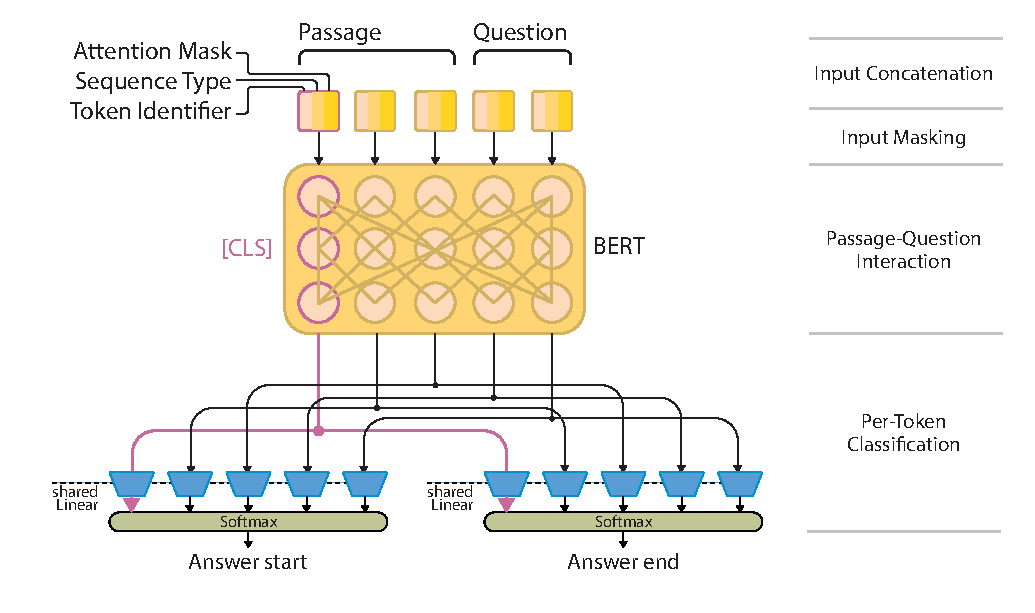
\includegraphics[width=\textwidth]{BERT_graph.eps}
\caption{BERT model for QA.} \label{fig_bert}
\end{figure}

\subsubsection{Implementation details}

After initial trial with a model from the Tensorflow Hub, we decide to move our implementation to the HuggingFace\huggingface transformers library~\cite{Huggingface}.

Huggingface is a fast evolving AI community which is very active in the field of NLP. They provide an easy-to-use framework for the use of transformers an relative tokenizers. Moreover, they host a huge collection of models, both pre-trained by them or by the fervent community.

We make use of transformers models and related tokenizers from the library.


\subsubsection{Experimental Setup and Results}

The HuggingFace setup allows us for fast swapping between language models. We conduct our runs with four models:

\begin{itemize}
\item BERT ~\cite{devlin2019bert}: this is the first contextual language model based on transformers. It achieves bidirectionality by training with the masked language model objective 
\item RoBERTa ~\cite{liu2019roberta}: a Robustly optimized BERT presents a slight modification in architecture by dropping the next sentence prediction objective and training the model with more data and compute.   %
\item ELECTRA  ~\cite{clark2020electra}is a more data and compute efficient method of training the transformer model: instead of masking 15\% of the words it corrupts the input by replacing tokens chosen among every one. The model then trains as a discriminator between correct and corrupted ones.
\item Longformer ~\cite{beltagy2020longformer}: this is a version of BERT able to process much longer inputs, it does so by adding sparse global attention on top of the 512 tokens long local attention of BERT.
\end{itemize}

We thus fine-tune BERT, RoBERTa, ELECTRA and the Longformer models on the QA task and compare their performance on the SQuAD v1.1 dev\_set with the official evaluation script.
\begin{table}[h]
\centering
\caption{Results for QA on SQuAD v1.1 Dev set with Transformers}\label{tab1}

\begin{tabular}{| c | c | c | c |}
\hline
Model &  Exact Match & F1-score & Inference Time\\
\hline
BERT &  70.45\% & 80.29\% & 206s \\

\hline
RoBERTa &  \textbf{83.95\%} & \textbf{90.59\%} & 207s\\

\hline
ELECTRA  small &  67.75\% & 77.76\% & 48s\\

\hline
Longformer &  82.74\% & 89.78\% & 1705s\\

\hline
\end{tabular}
\end{table}

\subsubsection{Analysis of results}

With our experiments we could clearly reproduce the improvements on transformer language model training that has been made after the publication of BERT.

The improvement in Exact Match given by the RoBERTa implementation is exciting. The authors showed how training expertise and data are crucial to squeeze the best performance out of a transformer architecture.

The Longformer architecture is promising in allowing the model to process much longer documents without quadratic increase in parameters and compute time over sequence length. However, this useful feature does not show its influence on our run. We speculate that this is the case because long passages are not really frequent in the SQuAD dataset (0.16\% of concatenated pairs exceeds 512 tokens in our training split).

Then, with ELECTRA the authors showed how to improve the resource efficiency in the training of transformers. This then results in better model scaling, especially for small models. 
ELECTRA shines by taking just 23\% inference time relative to original BERT. This makes it the perfect candidate for transformer based ranking for Information Retrival.

Finally, a comparison with our previous approach shows that the use of BERT-like question-passage encoding improves on the RNN baseline by a big margin. Although our RNN-attention network is nowhere near state-of-the-art (BiDAF reports an exact match of 68\% on the SQuAD leaderboard) this is a remarkable improvement over finely tweaked RNN models with just hours of BERT pre-tained weights fine-tuning.



\section{Information Retrieval}
Information retrieval or IR is the name of the field encompassing the retrieval of all manner of media based on user information needs~\cite{Woods1978SemanticsAQ}. In particular, in this work we focus on document retrieval given a text query. In our experimental setup the query is a question, while the documents are the text paragraphs where to look for the answer.


\subsection{Background}
The information retrieval task needed by QA consists into finding relevant pages in a database of documents given a query. This task is necessary for our open domain question answering since we need a fast reduction of data. Doing QA on the whole database would be time consuming and less precise. 
In this section we report the outcome of our experiments, which focus firstly on tf-idf, and then on a neural approach to the problem, leveraging on Transformers. The reason for which we are interested also in exploring the neural approach is that standard IR algorithms (like tf-idf or BM25) have long been known to have a conceptual flaw, known as the "vocabulary mismatch problem" ~\cite{Woods1978SemanticsAQ}: they work only if there is exact overlap of words between the query and the document. The idea is that by employing a neural architecture to perform IR we can hopefully overcome this issue, by producing dense embeddings instead of sparse word-count vectors. 
Due to our goal, namely linking the IR component to the best working QA architecture, we work with the SQuAD 1.1 dataset also in these experiments. In particular, we remove from SQuAD the answer-paragraph correspondences: the task of our IR models is then to find the right paragraph given a query (which in our case is the question itself).


\subsection{Metrics for IR}\label{metrics_IR}
Before presenting the two main architectures we explored in our research, it is important to describe the metrics we use to evaluate our IR systems. For this purpose we define some terms:

We define as \textbf{relevant document} the passages where the answer is present for a given question. 

We define as \textbf{retrieved documents} the passages returned from the information retrieval system.

We employ the Recall metric defined for information retrieval:

\begin{equation}\label{recall_eq}
\text{Recall}=\frac{|\{\text{relevant documents}\}\cap\{\text{retrieved documents}\}|}{|\{\text{relevant documents}\}|}
\end{equation}

This metric keeps track of the fraction of all relevant documents that are returned.

Another metric that suits our problem definition is the Mean Reciprocal Rank (MRR). MRR gives a general measure of quality for Information Retrieval systems with just one relevant result. It does so by weighting retrieved documents by their reciprocal position in the retrieved list.

\begin{equation}\label{mrr_eq}
{\text{MRR}}={\frac  {1}{|Q|}}\sum _{{i=1}}^{{|Q|}}{\frac  {1}{{\text{rank}}_{i}}}
\end{equation}

MRR is perfect for our system given that just one passage is relevant for each question in SQuAD.

In the next sections we describe our IR architectures and we provide the corresponding evaluations according to the abovementioned metrics, each of which evaluated for the top-k retrieved passages, for different k values.


\subsection{System Description: tf-idf}\label{tfidf section}

After performing a text pre-processing step as shown in section \ref{preprocessing_for_RNN} and splitting the \code{trainset} data in train and test sets, we use a tf-idf vectorizer to learn the vocabulary and the inverse document frequency, computing the document-term matrix on the training set. We find that the most effective configuration is to work with unigrams, while, contrary to what we expected, the stemming worsen the performances.
At this point we are able to transform all the test passages and questions to tf-idf weighted document-term matrices, by using the vocabulary and document frequencies learned on the training set. Then, we compute the cosine similarity between each question and passage sparse vector, obtaining a measure of how similar the two vectors are. By ranking all these values for a given question, we can extract the best match, which is the passage retrieved by our system.

\subsubsection{Experimental Setup and Results}
To evaluate the tf-idf approach we use the metrics introduced in section \ref{metrics_IR}.
The first metric we compute is the (average) recall (see equation \ref{recall_eq}), which concerns the fraction of all relevant passages that are returned. The second metric we compute is the MRR (see equation \ref{mrr_eq}), which instead shows what is the mean reciprocal rank of the relevant passage retrieved by the system after each query. In both cases the closer the outcome is to 1, the better the evaluated system is. 
The results obtained by applying these metrics to the top-k retrieved passages, for k values ranging from 1 to 10, are shown in figure \ref{IR metrics}.


\subsection{System Description: ELECTRA}
We proceed in our research by experimenting with an alternative to the presented tf-idf IR system. In particular, we focus on a neural approach based on a Transformer architecture. For all our experiments we choose to use ELECTRA small, a pre-trained Transformer model~\cite{clark2020electra}. This model has one main great feature: it has a lot less parameters with respect to BERT (13 millions vs 100 millions). Moreover, in ELECTRA the text encoder is pre-trained as a discriminator rather than as a generator and this strategy is much more efficient if compared to the standard Masking method used for BERT. Indeed, the discriminator task is defined over all input tokens rather than just on the small subset that was masked out. This leads to a model that despite being much smaller than BERT, can perform really well. For these reasons ELECTRA is probably the best fit for our experiments, because an important aspect to take into account when developing an IR system is its efficiency: the IR engine must indeed provide a result as fast as possible, and in a neural system we have to carefully find a trade off between performance and response time.


\subsubsection{Model}
The model is illustrated in figure: (\ref{fig_electra_IR}) and is constructed as follows:

\begin{enumerate}
  \item Questions and passages are pre-processed with the ELECTRA pre-processor
  \item Questions and passages are tokenized and padded separately. 
  \item Input passage and question are processed separately by the same ELECTRA model in a siamese training fashion.
  \item Sentence encoding for each input is extracted from the \code{CLS} token pooled output.
  \item Sentence encoding are further processed by two separate linear layers.
  \item Encodings are used to create the comparison matrix: each element is the dot product between a question and a passage representations.
  The main diagonal holds relevant pairs, while contrastive pairs from the batch fill the other positions.
  \item Softmax is performed on each row of the matrix, representing different passages for a given question.
\end{enumerate}

Training of the model is performed with the cross-entropy loss. This is applied to each row of the matrix and summed for every pair in the batch.
\begin{figure}[h]
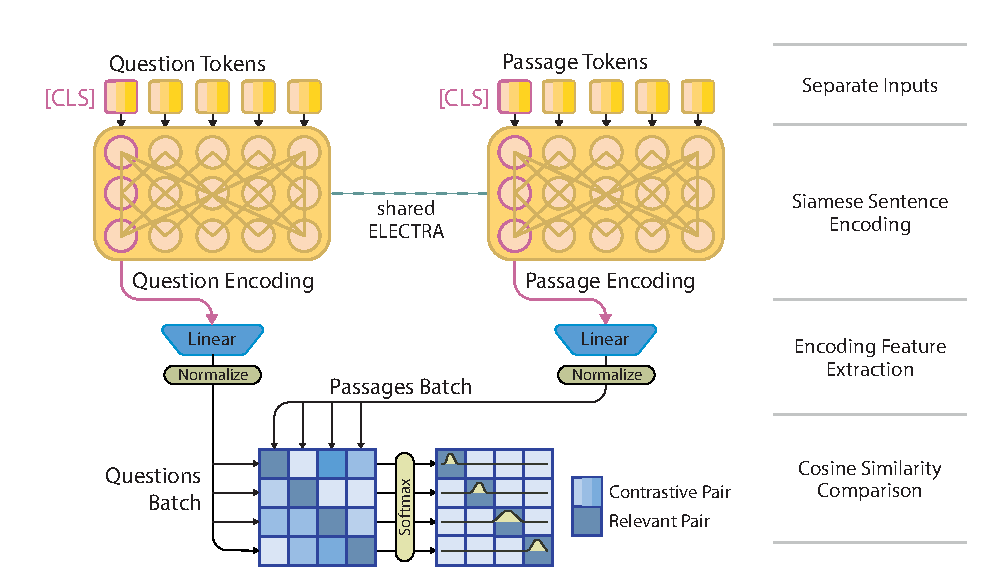
\includegraphics[width=\textwidth]{IR_ELECTRA_graph.eps}
\caption{ELECTRA model for Information Retrieval.} \label{fig_electra_IR}
\end{figure}

%%% rigirare
This network design aims to produce passage and question embeddings such that the cosine similarity between two corresponding representations will be higher than the similarity between unrelated question - passage pairs.
Another advantage is that thanks to this set-up we are able to encode all passages once and for all, before any query is submitted to the system. This way we can achieve a significant improvement in the efficiency of the IR component, because at inference time we just have to encode the question and search the nearest neighbours passage embedding according the cosine similarity metric.

\subsubsection{Experimental Setup and Results}

Training batches are constructed from \code{batch\_size} long pairs and we make sure to include in the same batch only passages that are different. This, together with the way the comparison matrix is constructed, ensures that the similarity between positive question-passage pairs appears only in the diagonal, while others values all correspond to negative pairs (meaning unrelated question-passage pairs).

We also test with hard negative mining of question-passage pairs: in this case a batch is constructed with passages from the same wikipedia page (found by title in the SQuAD dataset).
This strategy is quite intuitive: we force the network to learn to distinguish questions related to passages that are similar, establishing a more difficult, but pertinent, task to learn. However, we find that this prevents the model to train effectively. In our opinion, the questions in the considered dataset are too short and do not provide enough information to distinguish between similar passages.
For this reason we stick to the strategy intoduced at the beginning of this sub-section.

We make experiments with both siamese (shared weights) and separate training of the ELECTRA sentence encoders. 
With siamese training only one set of weights is saved, thus keeping the model small.
This however does not influence inference time, as both question and passage has to be processed anyway. 
These experiments with the separate training of two ELECTRA encoders (one dedicated to questions and one dedicated to passages) doesn't lead to improvements in the final results, so we decide to focus on the lighter siamese model.  

After training we evaluate the model pipeline on a held-out set of 10\% samples.

The metrics we use are the same employed for tf-idf and are the ones introduced in section \ref{metrics_IR}. The results obtained by applying these metrics to the top-k retrieved passages, for k values ranging from 1 to 10, are shown in figure \ref{IR metrics}.

\subsection{Analysis of results}
The results obtained by our IR systems can be compared by looking to figure \ref{IR metrics}. As we can see, the tf-idf approach outperformed the neural approach. We know for a fact that the classical Information Retrieval pipeline based on tf-idf is mature and largely used in this field: a survey conducted in 2015 showed that 83\% of text-based recommender systems in digital libraries use tf–idf~\cite{wiki_tf-idf}. On the other hand, IR approaches leveraging on dense vectors are an open research field, thus there's a lot of work to do, and it is quite hard (at least in this case) to reach the same performance of standard systems.
We make some hypotheses on why this task seems to be better suited for a standard tf-idf system with respect to a neural system. Our main hypothesis is that this is due to how the SQuAD dataset was created, namely by crowdsourcing: crowdworkers wrote down questions for different wikipedia pages and highlighted in those pages the corresponding answers. We think that this methodology "biases" in a way the crowdorkers towards writing down questions that will probably contain a lot of words also present in the corresponding passages, making this task incredibly well suited for the tf-idf system (which leverages on exact word matches between question and passage words). We also think that for a more general IR task in which the user has not read the document before writing down its query, it could happen to have a lot of mismatch between the query and the documents (for instance, the user could use synonyms of document words in the query), and this would be a task in which having a neural architecture would bring great performance improvements.

\begin{figure}
     \centering
     \begin{subfigure}[b]{0.49\textwidth}
         \centering
         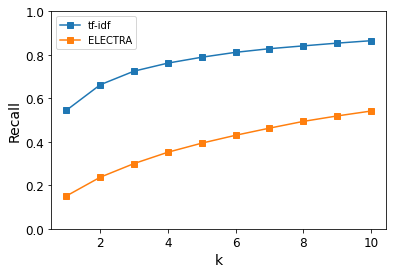
\includegraphics[width=\textwidth]{recall.png}
         \caption{Recall}
         \label{fig:metrics - recall}
     \end{subfigure}
     \hfill
     \begin{subfigure}[b]{0.49\textwidth}
         \centering
         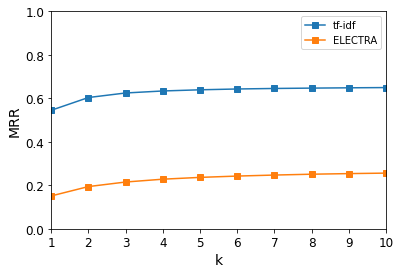
\includegraphics[width=\textwidth]{mrr.png}
         \caption{MRR}
         \label{fig:metrics - mrr}
     \end{subfigure}
     \hfill
        \caption{IR metrics comparison}
        \label{IR metrics}
\end{figure}

%%%%%%%%%%%%%%%%%%%%%%%%

\section{Deploy}
We decide to develop an end-to-end application able to perform factoid question answering on a broad selection of wikipedia pages related to a specific topic.
We use "Tom Cruise" as an example topic.

In order to deploy the end-to-end application several stages have to be taken into account:

\begin{itemize}
\item Wikipedia pages prefetch
\item Data preprocessing for both IR and QA
\item User interaction and question handling
\item Information Retrieval system to select valuable passages
\item Question Answering inference and answer extraction
\end{itemize}

\subsection{Initial steps}
The first component we implement in our system is the one that downloads all the Wikipedia pages related to the Tom Cruise filmography. Then a preprocessing step occurs, consisting of removing from the downloaded Wikipedia pages sections that are not relevant for our task and of preparing the text for the IR component.

\subsection{The IR component}
The adopted Information Retrieval strategy is to return the page most similar to the provided question. To achieve this we leverage on our best working IR system, namely the one based on tf-idf. The only difference with respect to the system we describe in section \ref{tfidf section} is that now the retrieval is performed on full length documents and not anymore on short passages. We decide to adopt this kind of strategy because experimentally it is the one that works the best. Indeed apparently the tf-idf IR component has less trouble in distinguishing between pages than between single passages. This makes sense, because each page contains a lot of information related to the page's topic, and this content is probably really different from the one of other pages. The same doesn't hold for single short passages, which span a restricted portion of the page's text. 
To assess our IR system performance on this slightly modified task, we decide to perform an additional test. In particular, we evaluate our tf-idf component trained on the SQuAD dataset on the task of full document retrieval (instead of passage retrieval), by using the metrics defined in section \ref{metrics_IR}. In other words, now we are satisfied if a passage from the same page of the true passage is returned (the SQuAD 1.1 dataset contains multiple passages for each Wikipedia page). The outcome of this evaluation (with the k parameter ranging from 1 to 10) is shown in fig \ref{IR doc metrics}.

From a practical view point at system startup each page is vectorized and stored in a memory structure. Then when a user make a query, the question is vectorized and it's performed the nearest neighbour search which rely on triangular inequality to reduce the search space.

At this point, the relevant document for the question has been identified and we can proceed by splitting the text in passages with a maximum length of 512 tokens, compatible with the Question Answering model input.

\subsection{The QA component: an initial prototype}
In our initial application prototype Question Answering was performed by the RoBERTa model trained on the SQuAD 1.1 dataset, the best among the described QA experiments. After the IR step, QA is performed on each passage from the retrieved wikipedia page: this usually results in 10-40 possible answers, but just one should be provided to the user. The inference probabilities of maximum start-end values are summed together for each passage, then used for ranking them among all the passages in the wikipedia page. The answer is selected from the best ranked passage.
With careful analysis we see that the correct answer is present among the provided ones, but is sometimes not the first one by probability.
We come to realize that our transformer implementations for QA have never really been trained with question-passage pairs where the passage was \textit{not} relevant to the question. This forces our QA component to find an answer in every presented passage, even if there isn't one.

\subsection{Training the QA Component on SQuAD V2.0}

Due to the reasons we just described, we decide to fine-tune the RoBERTa model on SQuAD v2.0, an augmented version of the dataset with more than 43k unanswerable questions. The case with no-answer in the passage is handled by returning the position of the first token \code{[CLS]} instead of any relevant token. The best passage is selected as the one holding the answer, or a no-answer message is provided to the user.

\begin{figure}
     \centering
     \begin{subfigure}[b]{0.49\textwidth}
         \centering
         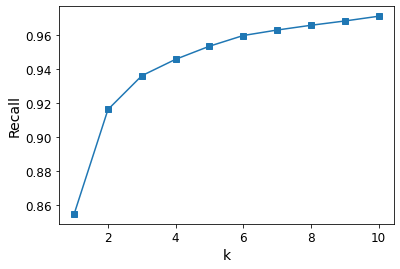
\includegraphics[width=\textwidth]{doc_recall.png}
         \caption{Recall}
         \label{fig:metrics - recall}
     \end{subfigure}
     \hfill
     \begin{subfigure}[b]{0.49\textwidth}
         \centering
         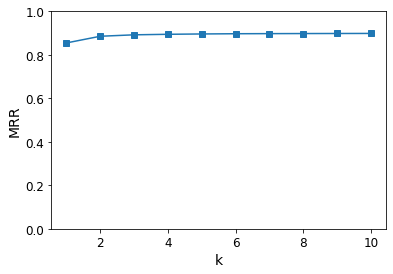
\includegraphics[width=\textwidth]{doc_mrr.png}
         \caption{MRR}
         \label{fig:metrics - mrr}
     \end{subfigure}
     \hfill
        \caption{tf-idf document metrics}
        \label{IR doc metrics}
\end{figure}


\subsection{The application}
We chose the web application format since it is extremely portable (a browser is enough) and a simple UI is easy to develop.
Another advantage is that the user questions (query) are handled using HTTP requests that are implementable in mobile applications or browser extensions, leaving the backend almost unchanged.

The different stages are executed in a distributed environment hosted on the Google Cloud virtual private cloud.


\subsection{Cloud architecture}
Google Cloud Platform provides an Infrastructure as a Service (IaaS) environment where to create and manage the necessary resources~\cite{wikiCloud}.
A production system has two main requirements: security and scalability.
Both of them must be handled by a careful cloud architecture design oriented to microservices.

\begin{figure}[h]
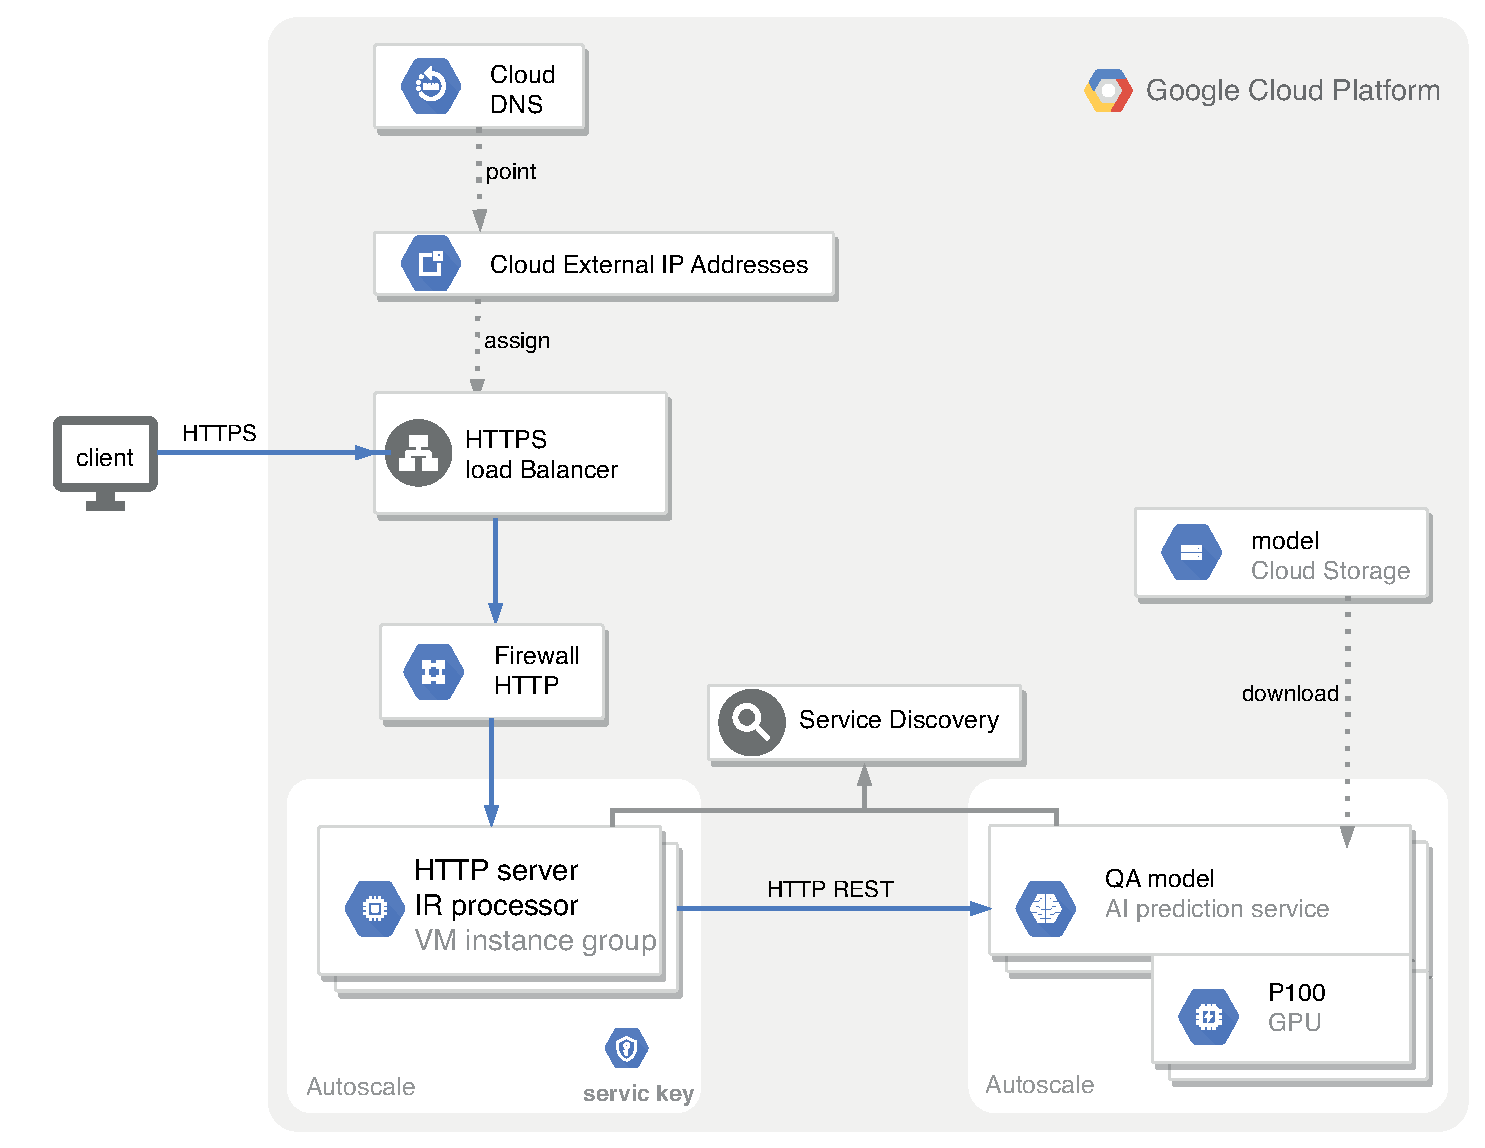
\includegraphics[width=\textwidth]{cloud_square.eps}
\caption{Cloud architecture } \label{cloud_arch}
\end{figure}

First of all the HTTPS protocol between the client and the server is mandatory to ensure confidentiality, while to grant server side authentication it has to provide a digital certificate signed by a Certificate Authority attesting the ownership of the domain name. 
The load balancer handles the HTTPS protocol and distributes the unencrypted incoming connection equally among the VMs in the Instance Group. The internal network allows only HTTP traffic coming from the load balancer as an additional security layer.

The backed Instance Group runs both the server and the IR processor and is configured to autoscale depending on the CPU usage. 
Each VM hosts an Apache2 server with the wsgi module enabled: this allows the execution of the python code that will preprocess the input and perform the IR task. The VM disk image also contains the Service Key needed to authenticate to the online prediction service.

Finally the question answering model, loaded to Cloud Storage, is deployed using the AI prediction service.
It consists in a cluster of machines equipped with the Tesla P100 GPU and configured to autoscale according to the workloads. 
The communication with the service happens through HTTP REST API and the Service Discovery takes care of the load balancing in a transparent way.

\begin{figure}[h]
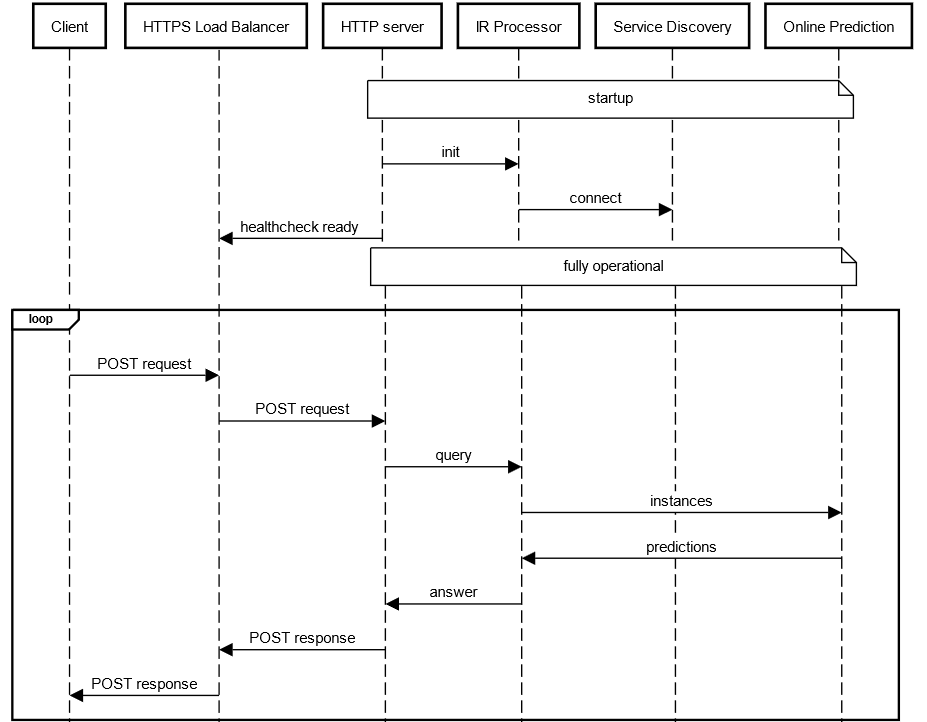
\includegraphics[width=\textwidth]{sequence.png}
\caption{Web App Sequence diagram} \label{seq_diag}
\end{figure}

The server initialization consists in preprocessing the wikipedia pages for both QA and IR tasks, splitting them in passages of compatible length with the QA model and then responding to the load balancer health-check as ready to receive requests.

For each query, the IR processor finds the document vector closest to the user question and then sends all the page’s passages to the Online Prediction service which return the raw probabilities.
Finally, the best prediction is selected and the answer text is decoded and presented to the user.


\pagebreak
\section{Discussion} 

In solving the Question Answering problem on SQuAD we experience how transformer based contextual language models have reached incredible performance as general pre-trainers for NLP tasks.
We show that we can reproduce this with relatively short fine-tuning of several BERT-like models.

We find that the ease of work with transformers is due to a mature community of researchers that share a common high-level framework mantained by Huggingface. This provides a vast  amount of costly pre-trained models free of charge.
We also couldn't have experimented so well without free GPU hours on Google Colaboratory.

Transformers work so well that performance on the SQuAD QA task has achieved above-human performance; this, however, does not mean that neural reading comprehension has been solved.
The task provided in the dataset is limited to factoid questions and the correct passage is already provided to the algorithm.
Nevertheless, the publication of SQuAD allowed for an advance in the NLP field in itself, and is still very relevant for evaluation of reading comprehension models.
\newline
\newline

The aim of our Information Retrieval work has been to design an end to end system that could retrieve Wikipedia passages to be fed to the QA reader for answer extraction.
For this reason we decide to continue using the SQuAD dataset for this task as it has been created on wikipedia.
We first develop a classical system that makes use of the term-frequency inverse-document-frequency well consolidated approach and see positive results.
We then want to incorporate the recent neural methods to improve on the task; following research on the topic we proceed by implementing our ELECTRA-based passage ranking model.
However, our experiments show that the performance of the baseline tf-idf is hard to reach. This should have its causes on the usage of SQuAD for the IR task. The Stanford dataset is small an not properly constructed for IR.
For this reason we think that further development of the project should consider the training on more recent datasets that are bigger and better suited for IR, such as MS MARCO~\cite{bajaj2018ms}or TREC~\cite{TREC}.
\newline
\newline

Following our development choices for QA and IR we show a complete end-to-end system for retrieval and reading of wikipedia pages for answer extraction.
The easy deploy is made possible by working on SQuAD with both systems.
Moreover, the streamlined Google Cloud Platform allows for easy implementation of all the technologies necessary for a solid web application to work.


\bibliographystyle{splncs04}
\bibliography{refs}


\end{document}

% TODO latex formatting:
% new paragraph without indentation
% clickable links with text not reference number
%TODO: dataset split

